\documentclass[a4paper, 12pt, final, openright, titlepage, twoside]{book}

%permette di aggiungere altri pacchetti dai file inclusi
\usepackage[subpreambles]{standalone} 


%impostazioni lingua
\usepackage[T1]{fontenc}
\usepackage[utf8]{inputenc}
\usepackage[english,italian]{babel}




\usepackage[dvipsnames]{xcolor}
\usepackage{graphicx}

\usepackage[italian]{varioref}

%sistema i margini
\usepackage{geometry}
\geometry{a4paper, top=2cm, bottom=2.1cm, inner=3cm, outer=2cm, heightrounded, foot=1.2cm}

%interlinea 1.5
\usepackage{setspace}
\onehalfspacing

%gestione delle testatine
\usepackage{fancyhdr}
\pagestyle{fancy}
\lhead{} \chead{} \rfoot{}
\rhead{} \lfoot{}
\cfoot{\thepage}
\renewcommand{\headrulewidth}{0pt}

%formattazione titoli paragrafo
\usepackage{titlesec}
\titleformat{\chapter}[display]{\normalfont\huge\bfseries}{Capitolo \thechapter}{0.7em}{\huge}

\usepackage{caption}

\usepackage{amsmath}

\usepackage{afterpage}


\usepackage[autostyle,italian=guillemets]{csquotes}
%sorting=nty per citazione in ordine di cognome, backref=true per mostrare dove una fonte è citata
\usepackage[sorting=none, style=numeric, citestyle=numeric-comp, backend=biber]{biblatex}

\addbibresource{bibliografia.bib}

%collegamenti ipertestuali
\usepackage[linktoc=all, colorlinks=true, allcolors=RoyalBlue]{hyperref}

%include il glossario

\usepackage[toc]{glossaries}

\makenoidxglossaries

% omozigosi/eterozigosi
% esoni
% ecotipo
% trasposone
% clade

\newglossaryentry{snd}{
	text={distribuzione normale asimmetrica},
	name={Distribuzione normale asimmetrica}, 
	description={TODO Una distribuzione normale asimmetrica.}
}

\newglossaryentry{dbn}{
	text={distribuzione binomiale negativa},
	name={Distribuzione binomiale negativa}, 
	description={TODO Una distribuzione.},
	plural={distribuzioni binomiali negative}
}

\newglossaryentry{dp}{
	text={distribuzione di Poisson},
	name={Distribuzione di Poisson}, 
	description={TODO Una distribuzione.},
	plural={distribuzioni di Poisson}
}

\newglossaryentry{db}{
	text={distribuzione binomiale},
	name={Distribuzione binomiale}, 
	description={TODO Una distribuzione.},
	plural={distribuzioni binomiali}
}

\newglossaryentry{locus}{
	text={locus},
	name={Locus}, 
	description={TODO Una distribuzione.},
	plural={loci}
}

\newglossaryentry{rate_eterozigosity}{
	text={rapporto di eterozigosi},
	name={Rapporto di eterozigosi}, 
	description={TODO Una distribuzione.},
	plural={rapporti di eterozigosi}
}

\newglossaryentry{assembly}{
	text={assembly},
	name={Assembly}, 
	description={TODO Una distribuzione.},
	plural={assembly}
}

\newglossaryentry{fitting}{
	text={fitting},
	name={Fitting}, 
	description={TODO Una distribuzione.},
	plural={fitting}
}

\newglossaryentry{snp}{
	text={SNP},
	name={SNP}, 
	description={TODO Una distribuzione.},
	plural={SNP}
}

\newglossaryentry{pcc}{
	text={coefficiente di correlazione di Pearson},
	name={Coefficiente di correlazione di Pearson}, 
	description={TODO Una distribuzione.},
	plural={coefficienti di correlazione di Pearson}
}


%genera testo casuale
\usepackage{lipsum}

\begin{document}
	
	
	\frontmatter
	\documentclass[crop=false]{standalone}

\usepackage[swapnames, norules, nouppercase, nowrite]{frontespizio}

\begin{document}
	\begin{frontespizio}
		\Istituzione{UNIVERSIT\`A DEGLI STUDI DI PADOVA \\ \vspace{1.5ex}}
		\Logo[3cm]{./resources/images/loghi.jpg}
		\Divisione{\textbf{Dipartimento di Ingegneria dell'Informazione} \vspace {2ex}}
		\Corso[Laurea]{\\ \vspace{0.5ex} \textbf{INGEGNERIA INFORMATICA}}
		\Titolo{\vspace{5cm}Stima della dimensione del genoma tramite k-mers:\\ confronto tra metodi computazionali.}
		\NCandidato{Laureando}
		\Candidato{Mattia Tamiazzo}
		\Relatore{Prof. Matteo Comin}
		\Rientro{1cm}
		\Piede {\vspace{1.5ex} \textmd{Data di laurea xx/09/2022} \\ \vspace{2ex} \vspace{1.5ex} Anno Accademico 2021-2022}
		\Preambolo{\renewcommand{\frontlogosep}{15pt}}
		\Margini{1.5cm}{1cm}{1.5cm}{1cm}
		\Preambolo{\renewcommand{\frontnamesfont}{%
				\fontsize{12}{14}\bfseries \vspace{4cm}}}
	\end{frontespizio}
	\cleardoublepage
\end{document}

	\documentclass[crop=false]{standalone}


\begin{document}
	
	\chapter*{\abstractname}
		La dimensione del genoma è la quantità totale di DNA nucleare aploide presente nelle cellule di un organismo. La determinazione della dimensione del genoma costituisce un argomento di interesse, perché non esistono valori di riferimento assoluti che permettano di stabilire quale approccio sia più efficace, e perché i metodi sperimentali per la sua misurazione sono attualmente costosi dal punto di vista temporale ed economico. Una soluzione alla stima della dimensione del genoma con metodi computazionali è l'utilizzo di k-mers, sottostringhe di DNA di lunghezza k. Questa trattazione si pone l'obiettivo di analizzare e comparare vari approcci algoritmici pubblicati in letteratura per la stima della dimensione del genoma, che tuttavia spesso forniscono risultati contrastanti e di difficile valutazione assoluta. Grazie ai limitati requisiti richiesti rispetto ai metodi attuali, comunque, la stima basata sui k-mer risulta essere un approccio promettente, anche per lo sviluppo futuro di metodi più precisi ed efficienti.
		
	\cleardoublepage
\end{document}

	\documentclass[crop=false]{standalone}

\setcounter{tocdepth}{1}

\begin{document}
	\hypersetup{linkcolor=black}
	\tableofcontents
\end{document}
	
	
	
	\mainmatter
	\documentclass[crop=false, class=book]{standalone}

\usepackage{lipsum}

\begin{document}
	\chapter{Introduzione}
	
	Il sequenziamento del DNA costituisce una tecnica fondamentale per lo studio del genoma di una specie, perché permette di determinare l'ordine delle basi azotate dei nucleotidi che costituiscono il DNA. Tale processo trova applicazione in molti studi biologici che riguardano vari ambiti, come ad esempio la medicina riproduttiva, l'oncologia o l'infettivologia, attraverso indagini tra cellule diverse dello stesso individuo o lo studio delle mutazioni genetiche tra individui di una stessa specie \cite{shendure2012expanding}. 
	
	% CONTENUTI (ordine da determinare)
	% a cosa serve (es: Assembly)
	% breve storia 
	% metodi (sperimentali vs computazionali) -> k-mer
	% cosa sono i k-mer
	
	\section{Storia}
	Lo studio approfondito del DNA si sviluppa a partire dal 1953, con la scoperta della sua struttura tridimensionale ad opera di James Watson e Francis Crick \cite{watson1953molecular}, contribuendo all'analisi dell'azione degli acidi nucleici nella sintesi proteica. Solo nel 1977 però, vennero sviluppate le prime strategie sperimentali per il sequenziamento, come il famoso metodo Sanger \cite{sanger1977DNA, sanger1977nucleotide} TODO
	
	
	\section{Sequenze di lunghezza k: i k-mer}
		TODO
		
	\subsection{K-mer profile}
	\label{subsec:kmerprofile}
	Il \textit{k-mer profile}, detto anche \textit{k-mer spectrum}, conta la frequenza dei k-mer trovati nelle letture di input, non assemblate o allineate. Esso può rappresentare un indicatore della complessità del genoma preso in esame \cite{vurture2017genomescope}, e mostra la quantità di k-mer distinti trovati ad una certa frequenza. Un esempio di k-mer profile è mostrato dalla figura~\vref{fig:profilecomp} tratta da \cite{sohn2016present}, in cui si può notare come la natura del genoma influenzi direttamente il grafico. 

	
	\begin{figure}
		\centering
		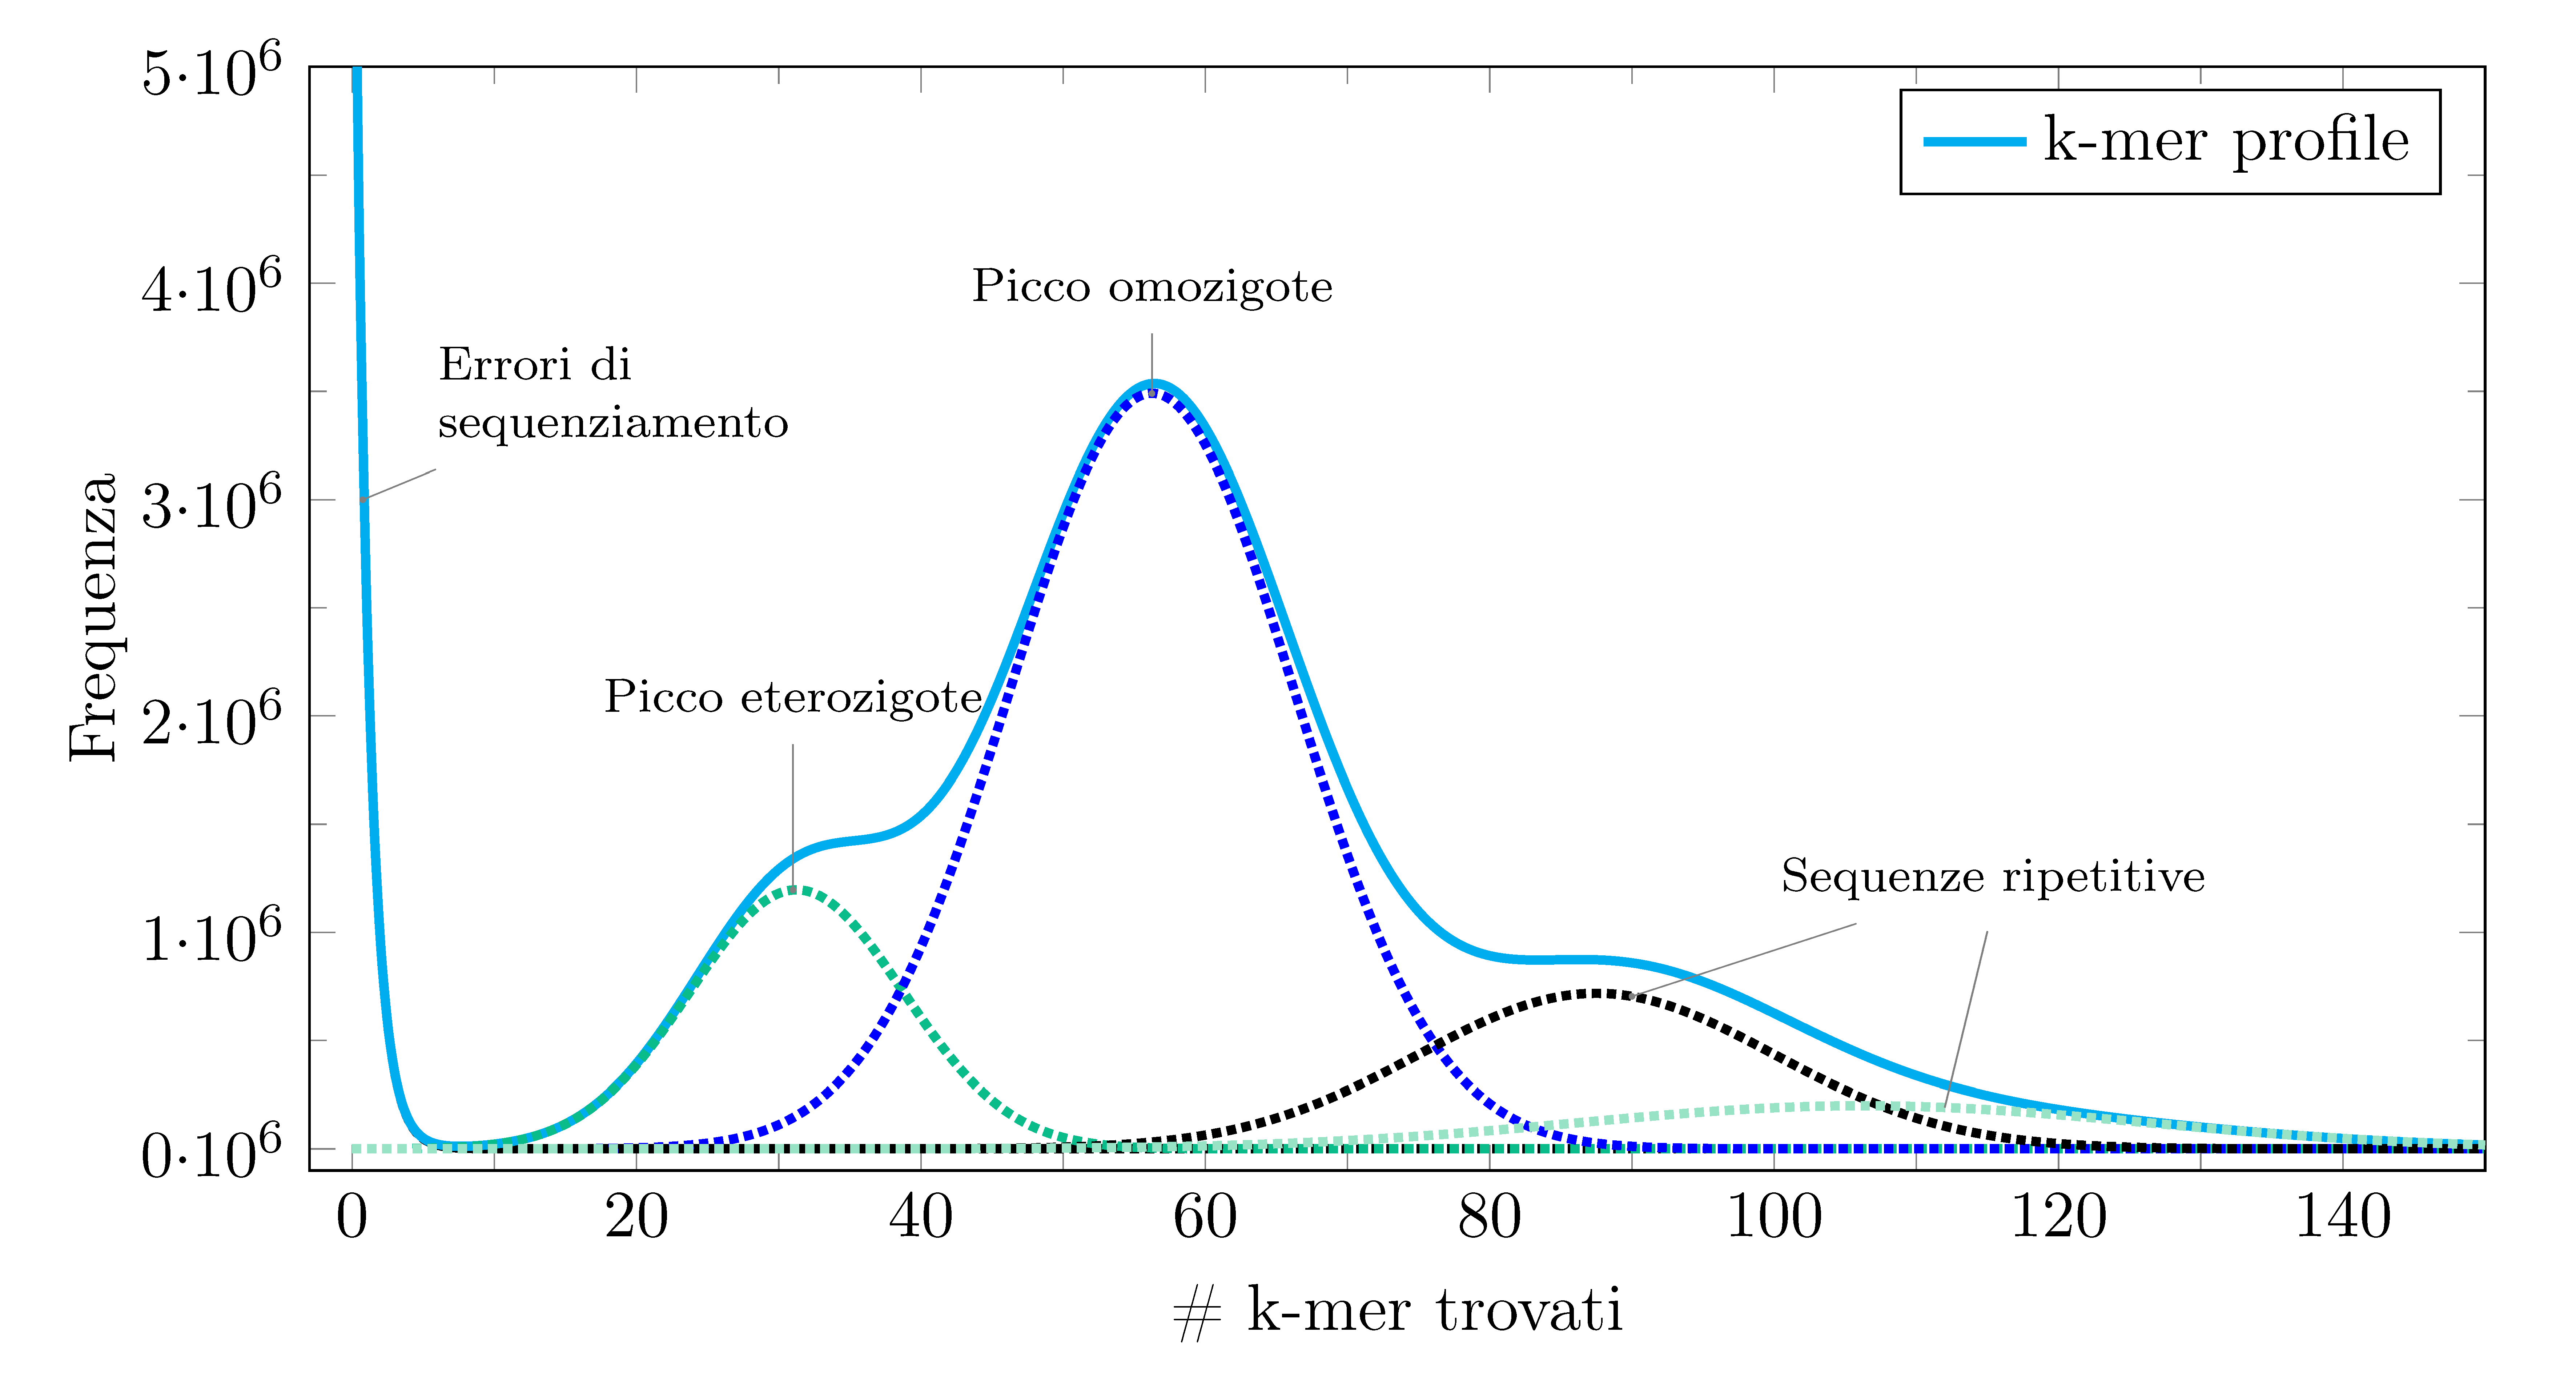
\includegraphics[width=0.8\textwidth]{capitoli/introduzione/profilecomp.png}
		\caption{TODO.}
		\label{fig:profilecomp}
	\end{figure}
	
	Ipotizzando che il genoma sia ideale, omozigote e senza ripetizioni, e che le letture siano state fatte senza errori con una certa copertura, il grafico del k-mer profile sarà una \gls{dp} centrata sulla copertura media disponibile.
	
	In casi reali invece, il genoma sarà eterozigote con una certa percentuale di eterozigosi e saranno presenti errori di sequenziamento; il k-mer profile presenterà tre picchi principali~\cite{sun2017findGSE}.
	Il primo picco del grafico corrisponde ai k-mer derivati da errori di sequenziamento, che accadono spesso ma che hanno bassa frequenza perché presentano poche occorrenze nelle letture di input; il secondo invece, rappresenta i k-mer eterozigoti e il terzo quelli omozigoti, presenti quindi su uno o entrambi gli alleli del set di cromosomi. I k-mer eterozigoti devono essere trattati più attentamente, perché possono risultare simili a quelli del primo picco, derivanti da errori di sequenziamento~\cite{sohn2016present}.	
	
	La lunga coda della distribuzione rappresenta invece le sequenze ripetitive, che occorrono con alta frequenza e sono presenti in un elevato numero di \gls{locus}. Eventuali ripetizioni aggiungono al grafico ulteriori picchi, mentre errori nelle letture aumentano la varianza e producono distorsioni nel grafico.
	
	La figura~\vref{fig:kmerprofile} mostra come all'aumentare del \gls{rate_eterozigosity} la quantità di k-mer eterozigoti del secondo picco diventi dominante rispetto ai k-mer omozigoti del terzo picco, che invece diminuiscono.
	
	Il k-mer profile può essere calcolato tramite programmi specifici date delle letture del genoma di input, quali \textit{Jellyfish}~\cite{marcais2011fast} o \textit{KMC2}~\cite{deorowicz2015KMC}.
	
	
	
	
	\begin{figure}
		\centering
		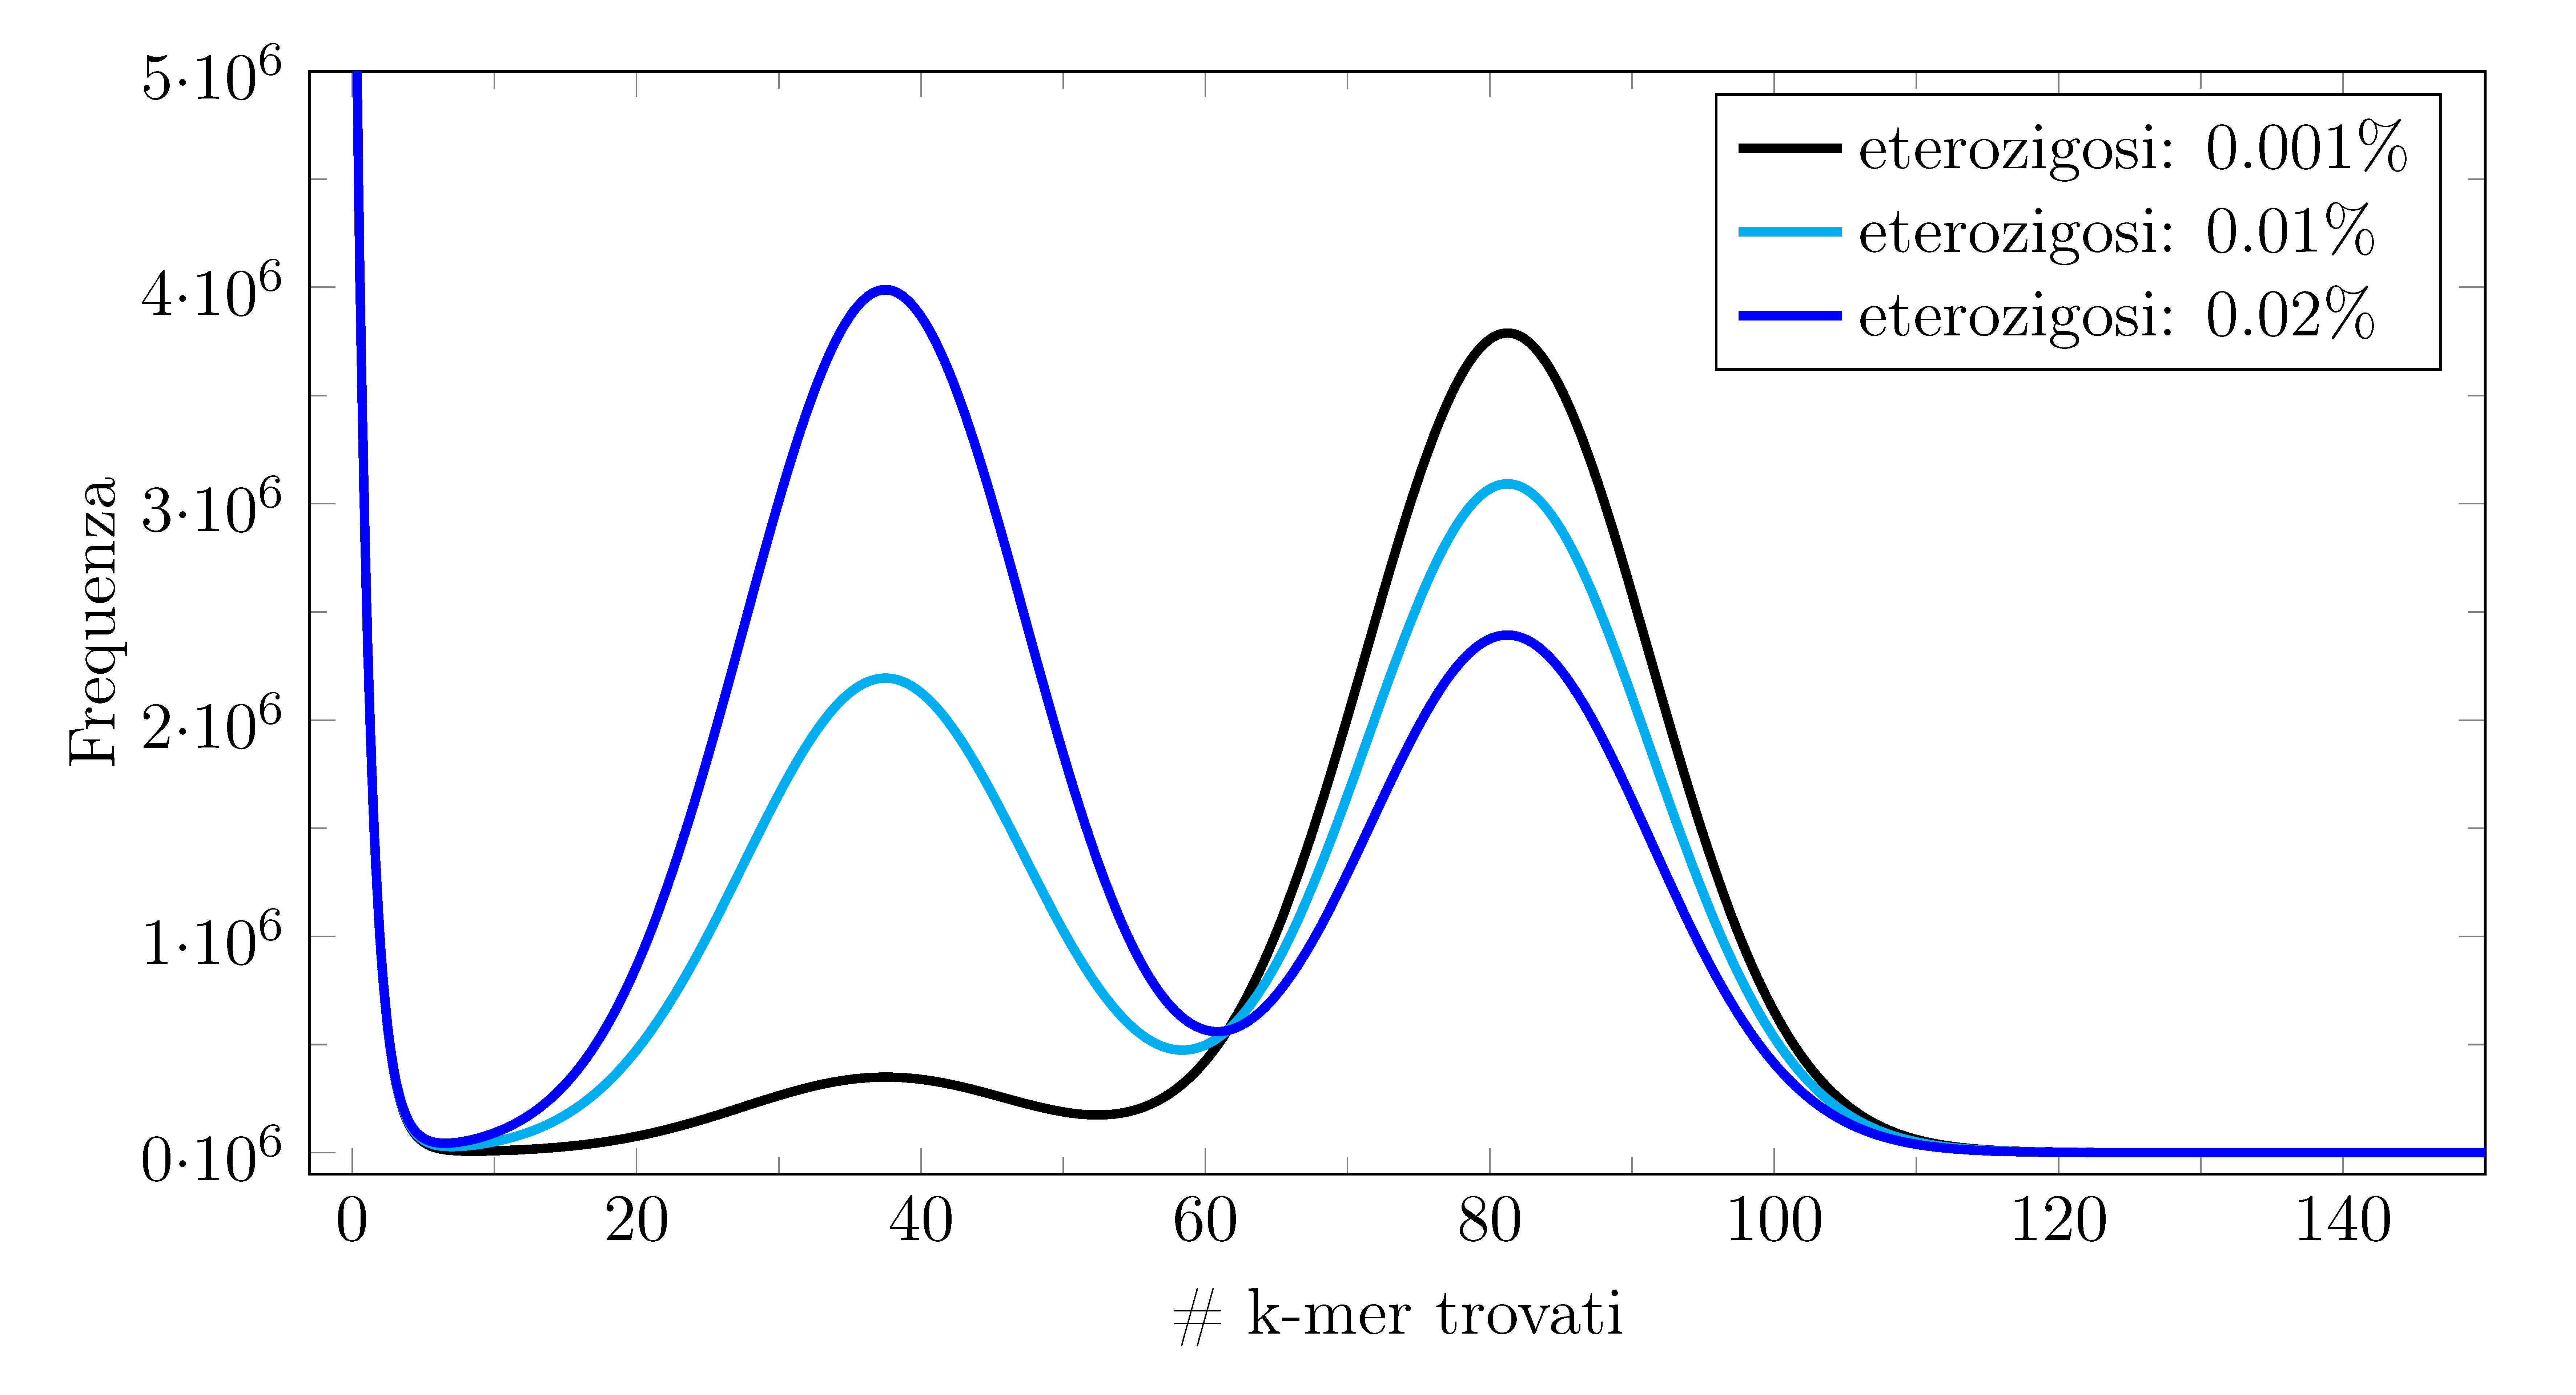
\includegraphics[width=0.8\textwidth]{capitoli/introduzione/kmerprofile.png}
		\caption{TODO.}
		\label{fig:kmerprofile}
	\end{figure}

	%\lipsum[1]
	%\section{Lorem ipsum}
	%\lipsum[2]
	%\subsection{Dolor sit amet} 
	%\lipsum[3]
	%\subsubsection{Lorem ipsum}
	%\lipsum[3]
	
	
	
	
\end{document}
	\documentclass[crop=false, class=book]{standalone}

\usepackage{lipsum}

\begin{document}
	\section{GenomeScope}
	
	Il progetto open source \textit{GenomeScope} cerca sia di stimare le caratteristiche del genoma completo, come la sua lunghezza o il rapporto di eterozigosi, sia di determinare le proprietà delle letture di DNA che prende in input, come la copertura (\textit{read coverage}) o l'error rate~\cite{vurture2017genomescope}. Il programma per determinare tali caratteristiche utilizza il k-mer profile del genoma preso in esame, descritto nella sezione~\vref{subsec:kmerprofile}.
		

	\subsection{Algoritmo}
	Il programma effettua una regressione non lineare dei dati iniziali, generando un profilo che cerca di approssimare il k-mer profile reale. Prendendo in input le letture del genoma che si vuole studiare, esso crea un modello che approssima il più possibile il k-mer profile. La funzione $f(X)$ scelta per l'interpolazione delle frequenze dei k-mer trovati è la somma di quattro \glspl{dbn} $Y \sim \mathcal{NB}(X;p,n)$, rispettivamente per rappresentare k-mer eterozigoti trovati nel genoma diploide una volta (unici) o tre volte (duplicati), e k-mer omozigoti di cui si trovano due occorrenze (unici) o trovati quattro volte (duplicati). La funzione $f(X)$ è descritta dall'equazione~\vref{eqn:gnmscp_regression}, in cui $G$ rappresenta un coefficiente di scala legato alla dimensione del genoma, $\lambda$ e $\rho$ sono rispettivamente la media e la varianza della distribuzione. 
	\begin{multline}
		f(X) = G \times (\alpha \mathcal{NB}(X;\lambda, \lambda/\rho) + \beta \mathcal{NB}(X;2\lambda, 2\lambda/\rho) + \\
		\gamma \mathcal{NB}(X;3\lambda, 3\lambda/\rho) + \delta \mathcal{NB}(X;4\lambda, 4\lambda/\rho)  ).	
		\label{eqn:gnmscp_regression}
	\end{multline}

	I coefficienti $\alpha, \beta, \gamma$ e $\delta$ dipendono dai parametri $r$ e $d$, che rappresentano rispettivamente il rapporto di eterozigosi, cioè la percentuale di basi che sono specifiche a uno o due cromosomi omologhi, e la percentuale del genoma che è presente in due copie.
	
	Lo scopo del programma è quindi determinare i coefficienti $r, d, \lambda$ e $\rho$, oltre alla dimensione totale del genoma $G$. La funzione scelta $f(X)$, tramite cui poi può essere calcolata la dimensione del genoma, è quella che restituisce la minore somma dei quadrati degli errori residui (\textit{Residual Sum of Square Error} - \textit{RSSE}), cioè che minimizzi la somma tra i quadrati degli errori tra i valori osservati e quelli stimati, come descritto dall'equazione~\vref{eqn:gnmscp_RSSE}. Per dedurre i valori dei coefficienti, viene utilizzata la funzione \verb|nls| del linguaggio di programmazione \textit{R}, che compie il \gls{fitting} dei dati alla funzione obiettivo.
	\begin{equation}
		RSSE = \sum_{x=E}^{+\infty} \left(kmer_{obs}[x] - kmer_{pred}[x]\right)^2.
	\label{eqn:gnmscp_RSSE}
	\end{equation}
	Al termine, il programma mostra all'utente i dati relativi al genoma trovati, come il rapporto di eterozigosi, la media e la varianza della distribuzione, l'indice RSSE, che rappresenta la percentuale di k-mer non considerati dal modello, e la dimensione stimata del genoma.
	
	La figura~\vref{fig:gnmscp_genomescopeprofile} mostra un confronto tra il k-mer profile reale e il modello costruito dal programma.
	
	\begin{figure}
		\centering
		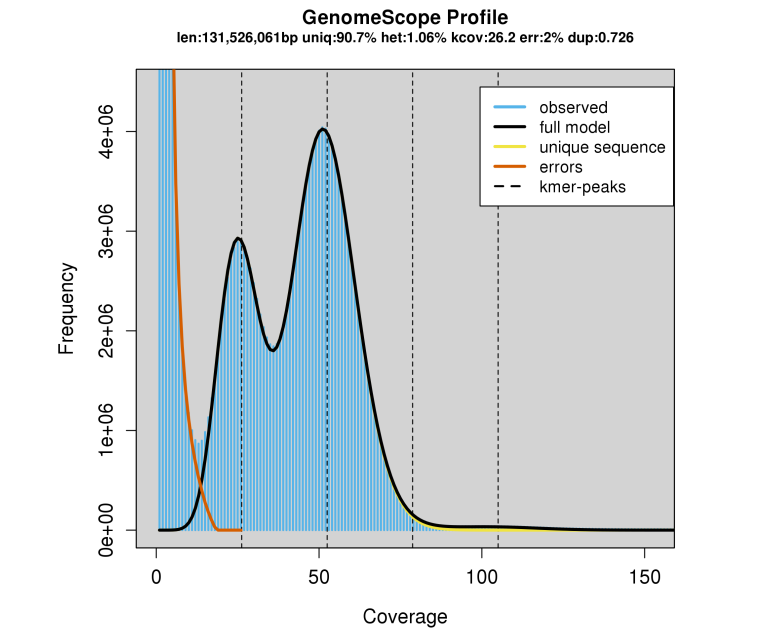
\includegraphics[width=0.6\textwidth]{capitoli/genomescope/gnmscp_genomescopeprofile.png}
		\caption{Modello del k-mer profile generato dal programma. L'istogramma in azzurro rappresenta i dati del k-mer profile reale, la curva nera il modello stimato e quella color arancione gli errori di sequenziamento stimati.}
		\label{fig:gnmscp_genomescopeprofile}
	\end{figure}


	\subsection{Gestione degli errori di sequenziamento}
	Eventuali errori di sequenziamento, ad esempio dovuti a duplicazioni con PCR o a sequenze contaminate, sono determinati solo empiricamente: dopo varie iterazioni del software in cui viene abbassata la soglia di copertura richiesta, i k-mer che non riescono ad essere rappresentati dal modello vengono identificati come errori di sequenziamento. 
	
	La stima dei k-mer sequenziati in modo errato è importante perché viene utilizzata per determinare la percentuale di basi errate nelle letture: una singola base inesatta infatti può dar luogo fino a $k$ k-mer errati, aumentando notevolmente il numero di errori. GenomeScope permette una percentuale $e$ di basi errate in ciascun k-mer. Tale valore è calcolato con un fitting dei k-mer errati a una distribuzione binomiale tramite la funzione \verb|uniroot| del linguaggio di programmazione \textit{R}. Questo metodo permette al programma di non dover assumere che la distribuzione degli errori di sequenziamento abbia una particolare forma, né di utilizzare un valore di soglia.
	
\end{document}
	\documentclass[crop=false, class=book]{standalone}

\usepackage{lipsum}

\begin{document}
	\section{findGSE}
	
	Il programma \textit{findGSE} \cite{sun2017findGSE} ha come obiettivo principale la stima della lunghezza del genoma. Utilizzando le frequenze dei k-mer trovati nelle letture a disposizione, il programma compie una regressione non lineare dei dati utilizzando come funzione una \gls{snd} (\textit{skew normal distribution} \cite{azzalini1985class,azzalini2005skew}).
	
	
	\subsection{Algoritmo}
	Nel programma viene assunto che le frequenze dei k-mer possano essere approssimate da una distribuzione normale asimmetrica $SN(\xi, \omega^2, \alpha)$. Presa in input la distribuzione delle frequenze dei k-mer (k-mer profile), l'algoritmo effettua la regressione determinando i quattro parametri che descrivono una distribuzione normale asimmetrica, la media $\xi$, la deviazione standard $\omega$, l'asimmetria $\alpha$ e un fattore di scala $s$. Ad ogni iterazione, il programma cerca di minimizzare l'errore tra i dati di input e la funzione stimata, in modo da approssimare il più possibile il k-mer profile reale. 
	
	Dato un genoma aploide con $G$ basi, il numero di k-mer possibili sarà $G-k+1$. Ponendo $C$ la copertura media dei k-mer, cioè che in media ogni k-mer sia trovato in $C$ letture diverse, e $N$ il numero di k-mer trovati nelle letture, la quantità di k-mer presenti nel genoma è descritta dall'equazione~\vref{eqn:findGSE1}. 	
	
	\begin{equation}
		\label{eqn:findGSE1}
		N=C \times (G-K+1)
	\end{equation}
		
	
	Posta la dimensione del genoma molto maggiore del numero di basi utilizzate $G\gg k$, l'equazione~\vref{eqn:findGSE2} approssima la dimensione totale del genoma in analisi.
	
	\begin{equation}
		\label{eqn:findGSE2}
		G\approx N/C
	\end{equation}

	A partire sia dal profilo reale che dal modello stimato, il programma calcola quindi il numero totale di k-mer trovati $N$ e la copertura media dei k-mer $C$, per poi calcolare la dimensione del genoma attraverso l'equazione~\vref{eqn:findGSE2}.
	TODO aggiungere qualcosa

	%TODO risultati?
	

	
	
	
\end{document}
	
	
	
	\backmatter
	\documentclass[crop=false]{standalone}

\begin{document}

	\printnoidxglossary[sort=word, style=list]

\end{document}
	
	\documentclass[crop=false]{standalone}

\usepackage[autostyle,italian=guillemets]{csquotes}
\usepackage[style=numeric,citestyle=numeric-comp,backend=biber]{biblatex}

\addbibresource{bibliografia.bib}

\begin{document}
	\printbibliography[heading=bibintoc]
\end{document}
	
	
\end{document}
